\section{Implementation of Scratch Detector}
In this chapter the development and results of a YOLOv5 solution for detection of scratches found on printed layers of a 3D binder jet printer. The following subsections will extend and go in-depth on the list of challenges presented in TODO and present solutions and ideas to handle them.

\subsection{Development Environment \& Setup}
TODO draft available, write it at the end

\subsection{Labeling the Dataset}
TODO: verallgemeinern mit scratches \\

\textbf{The first challenge:}
As mentioned \ref{intro:challenges}, some scratches are weaker and should not be marked as actual scratches to not make the model too sensitive. A sensitive model would lead to many false positive detections like a thicker edge or an oxidation spot. The main goal would be to find a metric that can evaluate the prominence of the scratches. With such a metric, each annotated scratch will have a prominence value and therefore a minimum threshold could be used to eliminate the weaker scratches.

\textbf{The solution:}
A proper metric should measure how dark a scratch line is with respect to it's neighboring background. Also, the metric should not take in consideration the length or width of the scratch.
The metric developed for this project works as follows:
Crop the bounding box from the image. Because the image is a grayscale, the cropped image will have only 1 channel i.e. it can be interpreted as a 2D array. The rows of the array are normalized and the mean row is then calculated. For clarification: the mean row is obtained by summing all rows into 1 row and dividing each element of that row by the total number of rows. The center values of the mean row are usually lower than the values from the start or end of the mean row, because the bounding box has the scratch with darker pixels positioned in the center. The plot of the mean row would look like the hyperbole of $f(x)=x^2$. The mean row is then multiplied by -1 and the plot would look more similar to $f(x)=-x^2$. This mean row multiplied by -1 can be interpreted as single pulse of a signal and the prominence of this signal pulse can be calculated by using special signal processing functions like TODO. \\
TODO figure of metric here. \\

Darker scratches will tend to have a higher prominence value than the faded ones. Now the only thing left to do is to choose a threshold and filter out the weak scratches. \\
During the filtering process, it was obeserved that some scratches had a surprisingly low prominence value. Usually, this was because the bounding box was not properly sized and the edges of a printed part were contained. Because the edges are dark, this would make the signal curve flatter and therefore the prominence value would be smaller. A resizing or centering of the bounding box solved this problem.

TOOD figure of bb with edges here. \\


\subsection{Bitmask Integration}

\textbf{The challenge:}
As discussed in TODO, the images of the layers have two types of anomalies:
\begin{enumerate}
\item thick edges or closely positioned segments that look like scratches
\item artifacts from previous layer that look like scratches
\end{enumerate}

This situations might trick even humans and during labeling it was found out that each potential scratch had to be checked by looking the current bitmask and the previous bitmask. The current bitmask was used to check against the first type of anomalies and the previous one for the second type of anomalies. This lead to the intuition of integrating the bitmasks in the training process.
 However, most object detectors take as input exactly one image with the respective annotations. The challenge is to find a proper way to integrate the two bitmasks with each image and provide the model this extra context information.


\begin{figure}[ht]
  \centering

  \begin{subfigure}{0.75\textwidth}
    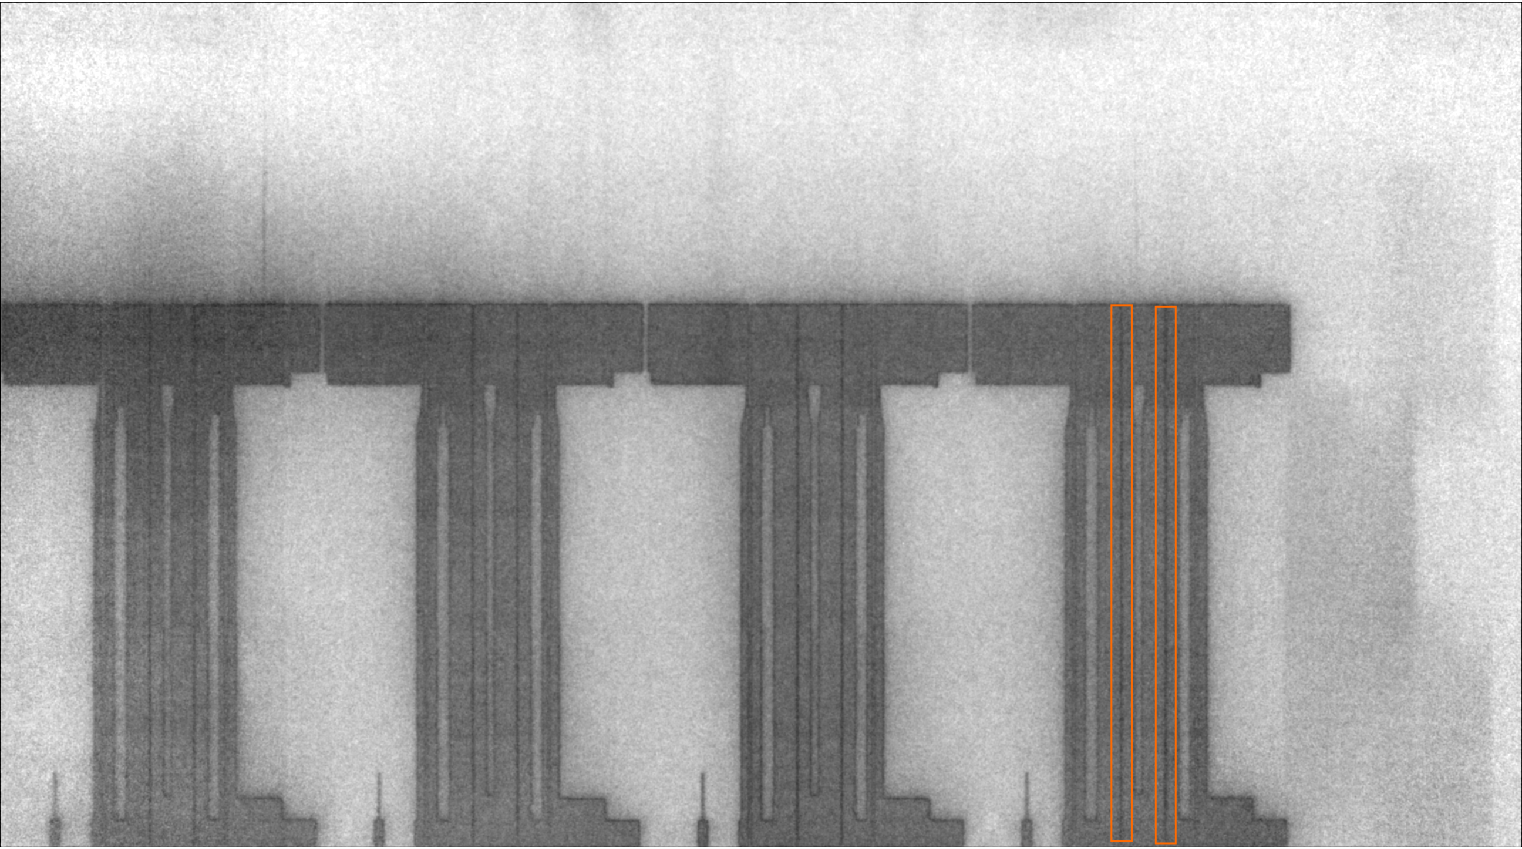
\includegraphics[width=\textwidth]{images/layer_01486_marked}
    \caption{Layer with thin splits marked in orange bounding boxes.}

  \end{subfigure}

  \begin{subfigure}{0.75\textwidth}
    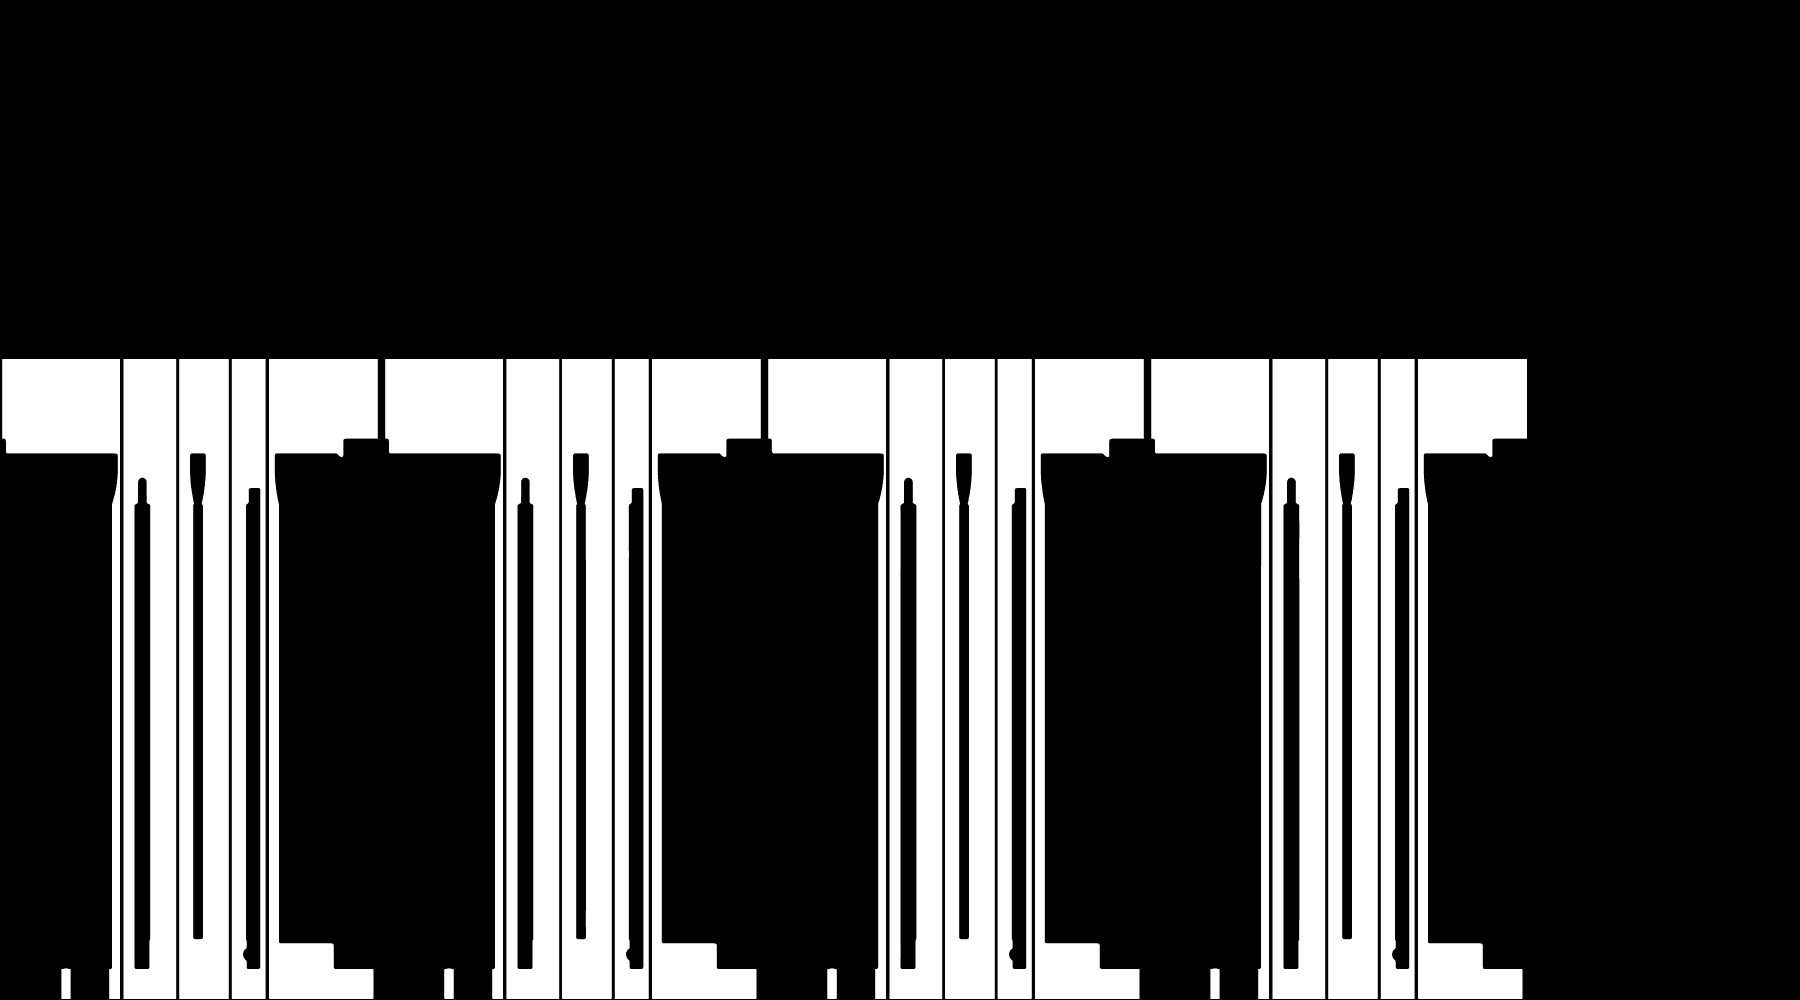
\includegraphics[width=\textwidth]{images/bitmask_01486}
    \caption{Corresponding bitmask must be checked to see if it's a scratch or a thin split.}
  \end{subfigure}

  \caption{Thin splits. TODO horizontal allign, better images}
  \label{fig:thin_splits}

\end{figure}

\textbf{The solution:}
YOLOv5 works with RGB images and if a grayscale input image is detected, it gets converted to RGB. This conversion provides no extra information and is more a preprocessing step. An alternative conversion method is to represent the grayscale with a single channel only e.g. the red one and the other two channels are just some blank images. \\

TODO figure with the conversion methods. \\

The second conversion methods will free up two channels that can be used to add relevant context information. With the challenge statement in mind, filling up the other two channels with the current and previous bitmasks is clearly helpful e.g. the green channel contains now the current bitmask and the blue channel contains now the previous bitmask. This is possible, because the bitmask images are also grayscale images. So instead of provding a grayscale image as an RGB image, three grayscle images are provided as an RGB image. \\

TODO figure to show new image mode \\

This new type of input image proved to make the model more robust against the above described anomalies, but with this new input some consideration and adaptations need to be made. \\
The layer images and the bitmask images have the same ratio, but different sizes of respectively 2592x1440 and 1800x1000. On one hand, the layer images can be downscaled to 1800x1000 and some image information is lost. On the other hand, the bitmask can be upscaled and the pixel-perfect edges get blurred. Another approach would be to meet somewhere in between e.g. downscale the layer images to 2196x1220 and upscale the bitmasks to 2196x1220. This tradeoff can be however avoided, if the the bitmasks are upscaled to the resolution of the layer images and a threshold on pixel values is used i.e. the pixels with a value below 0.5 are set to 0 and the rest are set to 1. The upscaled and thresholded bitmasks will retain this way all the pixel precise context informations.  \\
Now the inference step will also need an extra preprocessing step to include the bitmasks and without them the inference is invalid. Also, the first layer is a special case, because it does not have a previous bitmask and the current layer is inserted twice. \\
This concept of filling the channels with context informations was tested under many variations, but the one presented above delivered the best result. Most variations kept the original input image as the first channel and used different ways to fill up the other two channels. Some example of variations are:
\begin{itemize}
\item layer image and twice the current bitmask
\item layer image,the current bitmask and a logical OR of the current and previous bitmasks
\item layer image, the current Sobel-filtered bitmask and the previous bitmask
\end{itemize}
The first example does not include any informations about the previous bitmask, so the second type of anomalies, the artifacts from previous layers, are detected as edges. The second example was problematic in some cases, because a logical OR of two bitmasks might treat a gap between two segments from the previous layer as a printed region. This leads to detecting a thin gap as a scratch. In the third example the initial intuition was that a Sobel-filter will directly show where the edges are, but the problem is that information about the current printed regions is lost. The list of variations is long, but those were some examplesto get an intuition how context information is lost or malformed.





\subsection{Augmentations}
TODO: muss ich sagen woher ideal dataset? \\
The dataset at hand features a total of 2295 images of layers with the corresponding bitmask, but only a fraction of the images contain an actual scratch. This makes the dataset from the recommended minimum of 1500 images per class and 10000 instances per class. This forced a focus shift on augmentation methods. \\
When it came to evaluating an augmentation method, identical dataset shuffles (train, validation, test splits) were used for multiple reasons. One reason is that it's easier to visually compare the validation errors, if the exact same image is used. One nice feature supported with Weights \& Biases logger is the Bounding Box Debugger, which lets the user see the validation labels for each epoch for multiple runs. If the runs had the exact same validation images, then a head-to-head comparison was possible.\\

\begin{sidewaysfigure}
    \centering
    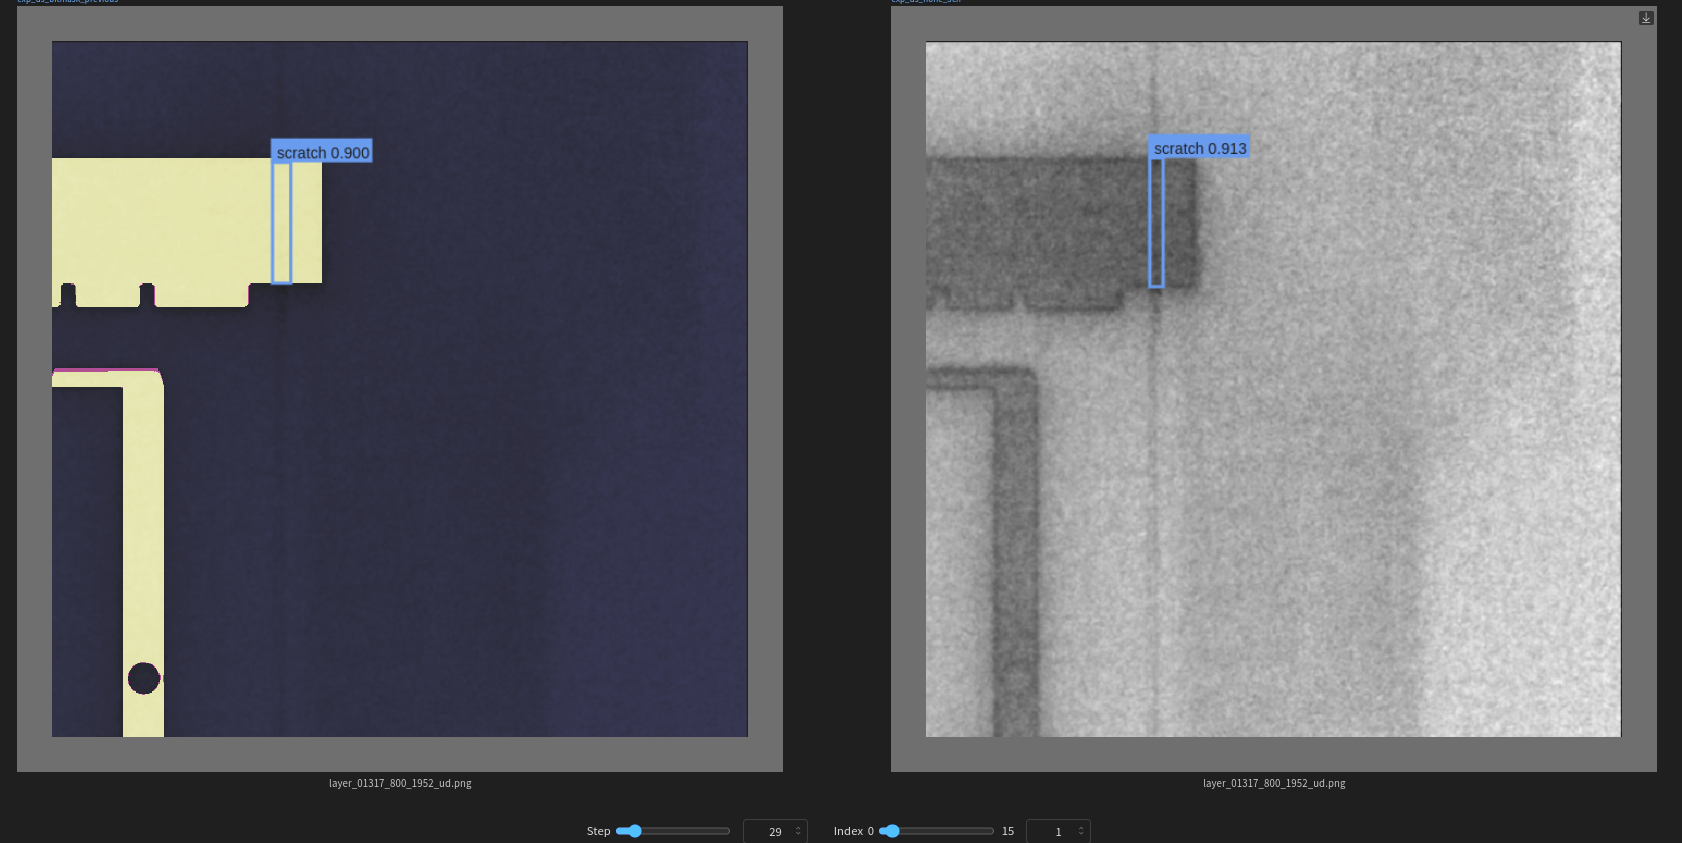
\includegraphics[width=\textwidth]{images/bb_debugger}
    \caption{Comparing head-to-head detections on validation images with the Bounding Box Debugger}
    \label{fig:bb_deb}
\end{sidewaysfigure}

Another reason for using identical shuffles is that in small datasets, shuffles are game of chance in terms of data variety. So, when using an identical shuffle, the same variety is ensured. TODO: maybe delete or reformulate this. \\


\subsection{Windowing}
One of the most analyzed and exhaustively tested augmentation method is the windowing method. This method simply takes a rolling window over the image and splits the images in smaller crops, called windows. First, some initial remarks will be presented.
\begin{itemize}
\item \textbf{Less CUDA memory:} The training process will now use smaller images, so there will more CUDA memory available, which means a bigger batch size is possbile.
\item \textbf{Bounding box conversion:} The bounding boxes need to be adjusted to the new window. Luckily, the albumentations library cropping methods supports this.
\item \textbf{Square vs rectangular training:} The initial intuition was to use tall rectangular windows, that can contain even the longer scratches. This way, the risk of obtaining tiny parts of a scratch in a window was avoided. However, YOLOv5 dataloader support shuffling only for square input images, which in some initial experiments showed a great improvement. Also, the cropping methods from albumentations support filtering tiny bounding boxes.
\item \textbf{Training times:} After splitting the data into windows, a lot of background windows (i.e. windows that do not contain scratches) are obtained, which can be filtered from the dataset. If not mentioned otherwise, all the background images/windows are removed from the dataset. This greatly improves training times by showing to the model only relevant sections of layers that contain scratches. YOLOv5 documentation recommends about 0-10\% background images. Also, images of smaller resolution take less time to be processed.
\item \textbf{Window overlapping:} In some unlucky cases a scratch might land on the edge of a window. To avoid this situation, all neighbouring windows have an overlap between them.
\end{itemize}

\subsubsection{Windowing Strategy}
The first window strategy, called \textit{grid windowing}, used to extract windows at the same positions for each layer. This showed great results, but a potential problem was that some consecutive layers had the scratches at the exact same locations. This lead to the development of \textit{random windowing}, which crops 1-2 random windows containing each scratch. In this way, the series of similar layers with repeating scratches was diversified into windows that contained the scratches at different positions. However, this method was sometimes unstable. The key difference is that at \textit{grid windowing} a scratch could be captured in 2 neighboring windows due to the overlap and this way the same scratch was captured in twice but at different positions at the window. At \textit{random windowing} this effect could be simulated by taking a random window of the scratch twice, but there was no guarantee that the windows capture the scratch in 2 different perspective. The randomness of this strategy could of course be improved, but it was not worth the effort since \textit{grid windowing} does it good enough. TODO explain better. TODO insert image explaining this concept. In figure \ref{fig:win_strategy} the windows of both methods can be visualized.  TODO: maybe try on second dataset.

\begin{figure}
  \begin{center}
  \begin{tabular}{ c c c }
  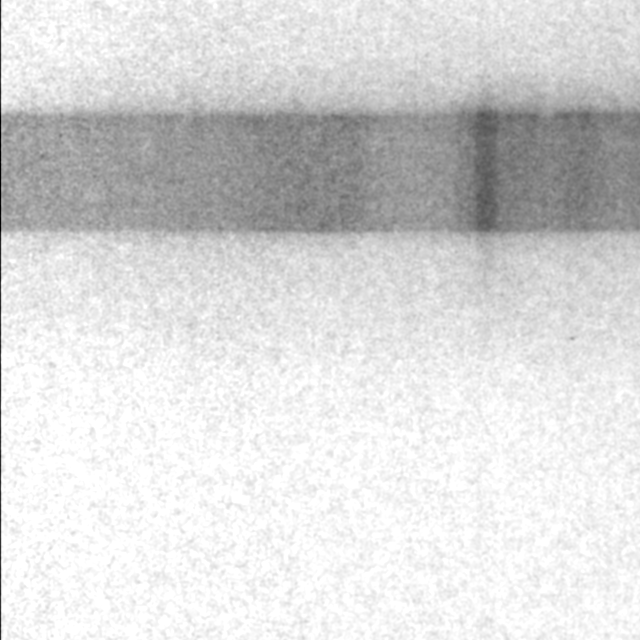
\includegraphics[width=.3\linewidth]{images/win_strategy/layer_21_grid} &
  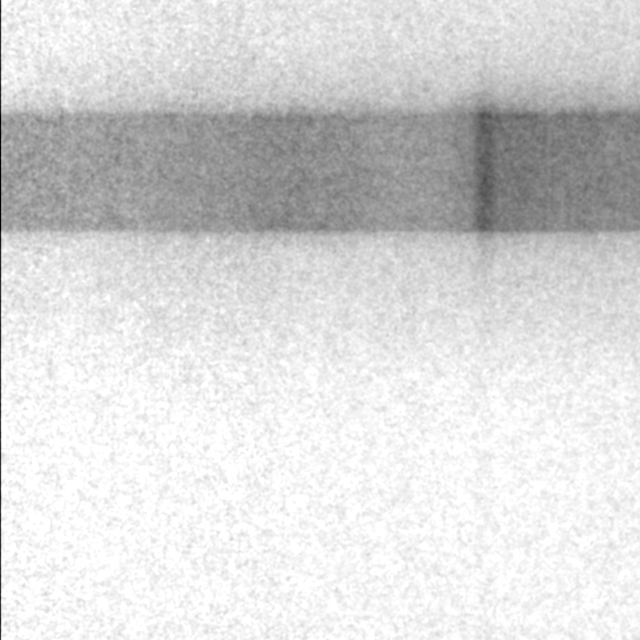
\includegraphics[width=.3\linewidth]{images/win_strategy/layer_22_grid} &
  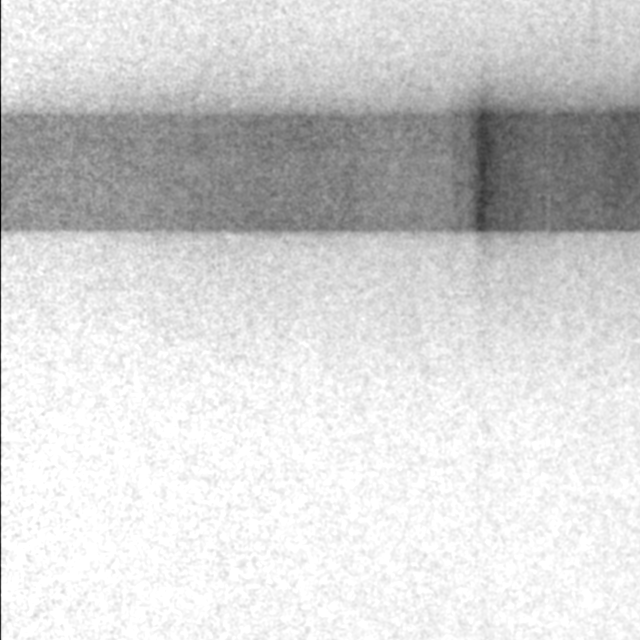
\includegraphics[width=.3\linewidth]{images/win_strategy/layer_23_grid} \\
   & & \\
  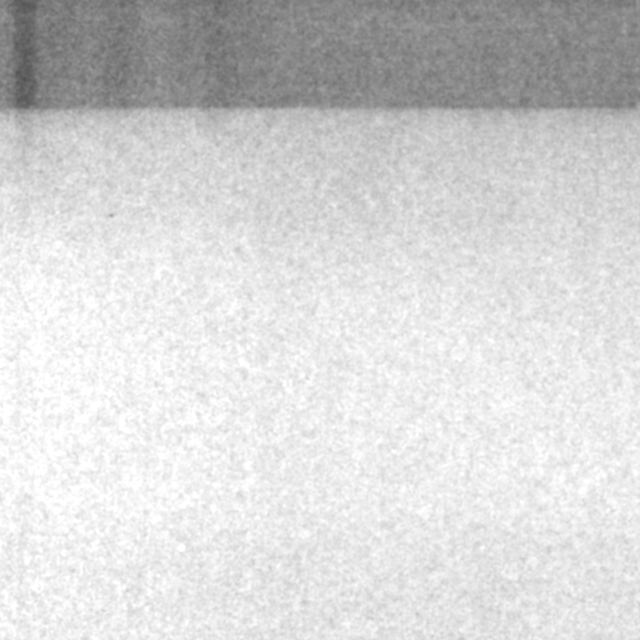
\includegraphics[width=.3\linewidth]{images/win_strategy/layer_21_rand} &
  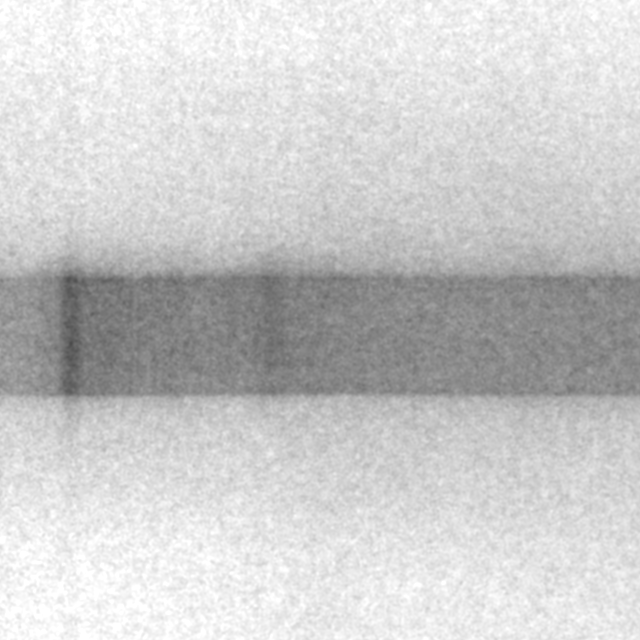
\includegraphics[width=.3\linewidth]{images/win_strategy/layer_22_rand} &
  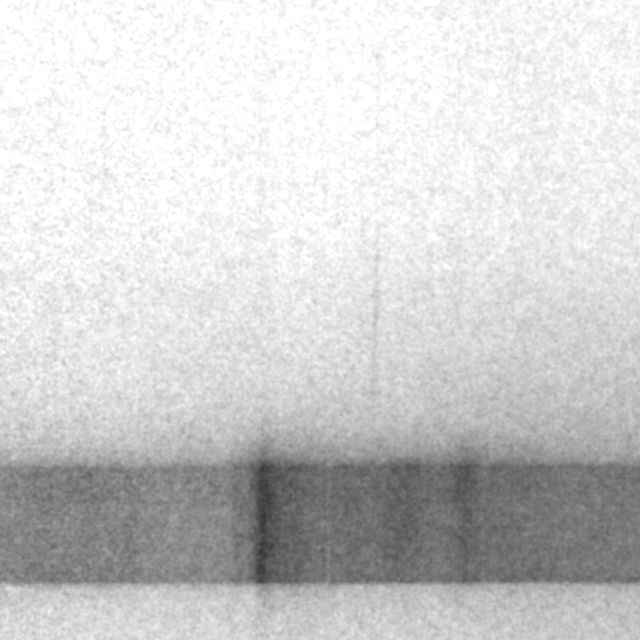
\includegraphics[width=.3\linewidth]{images/win_strategy/layer_23_rand} \\
  \end{tabular}
  \end{center}

  \caption{An exmample of the windowing strategies on 3 similar layers with repeating scratches. The first row shows the grid windowing method and the second row shows the random windowing method.}
  \label{fig:win_strategy}
\end{figure}

\subsubsection{Window Size}
For testing the effects of the window size, YOLOv5 has been trained on datasets with window sizes of 320, 640, 960 and 1280. The single constraint imposed by YOLO detectors is that the height and width needs to be a multiple of 32. \\
When it comes to better metrics, bigger windows got the better results. The intuitive explanation is that a bigger window may contain not only the annotated scratch itself, but also other dark lines that mimic a scratch like the thin splits shown in figures \ref{fig:thin_splits}, \ref{fig:thin_splits_previous_layer}.\\

\begin{figure}
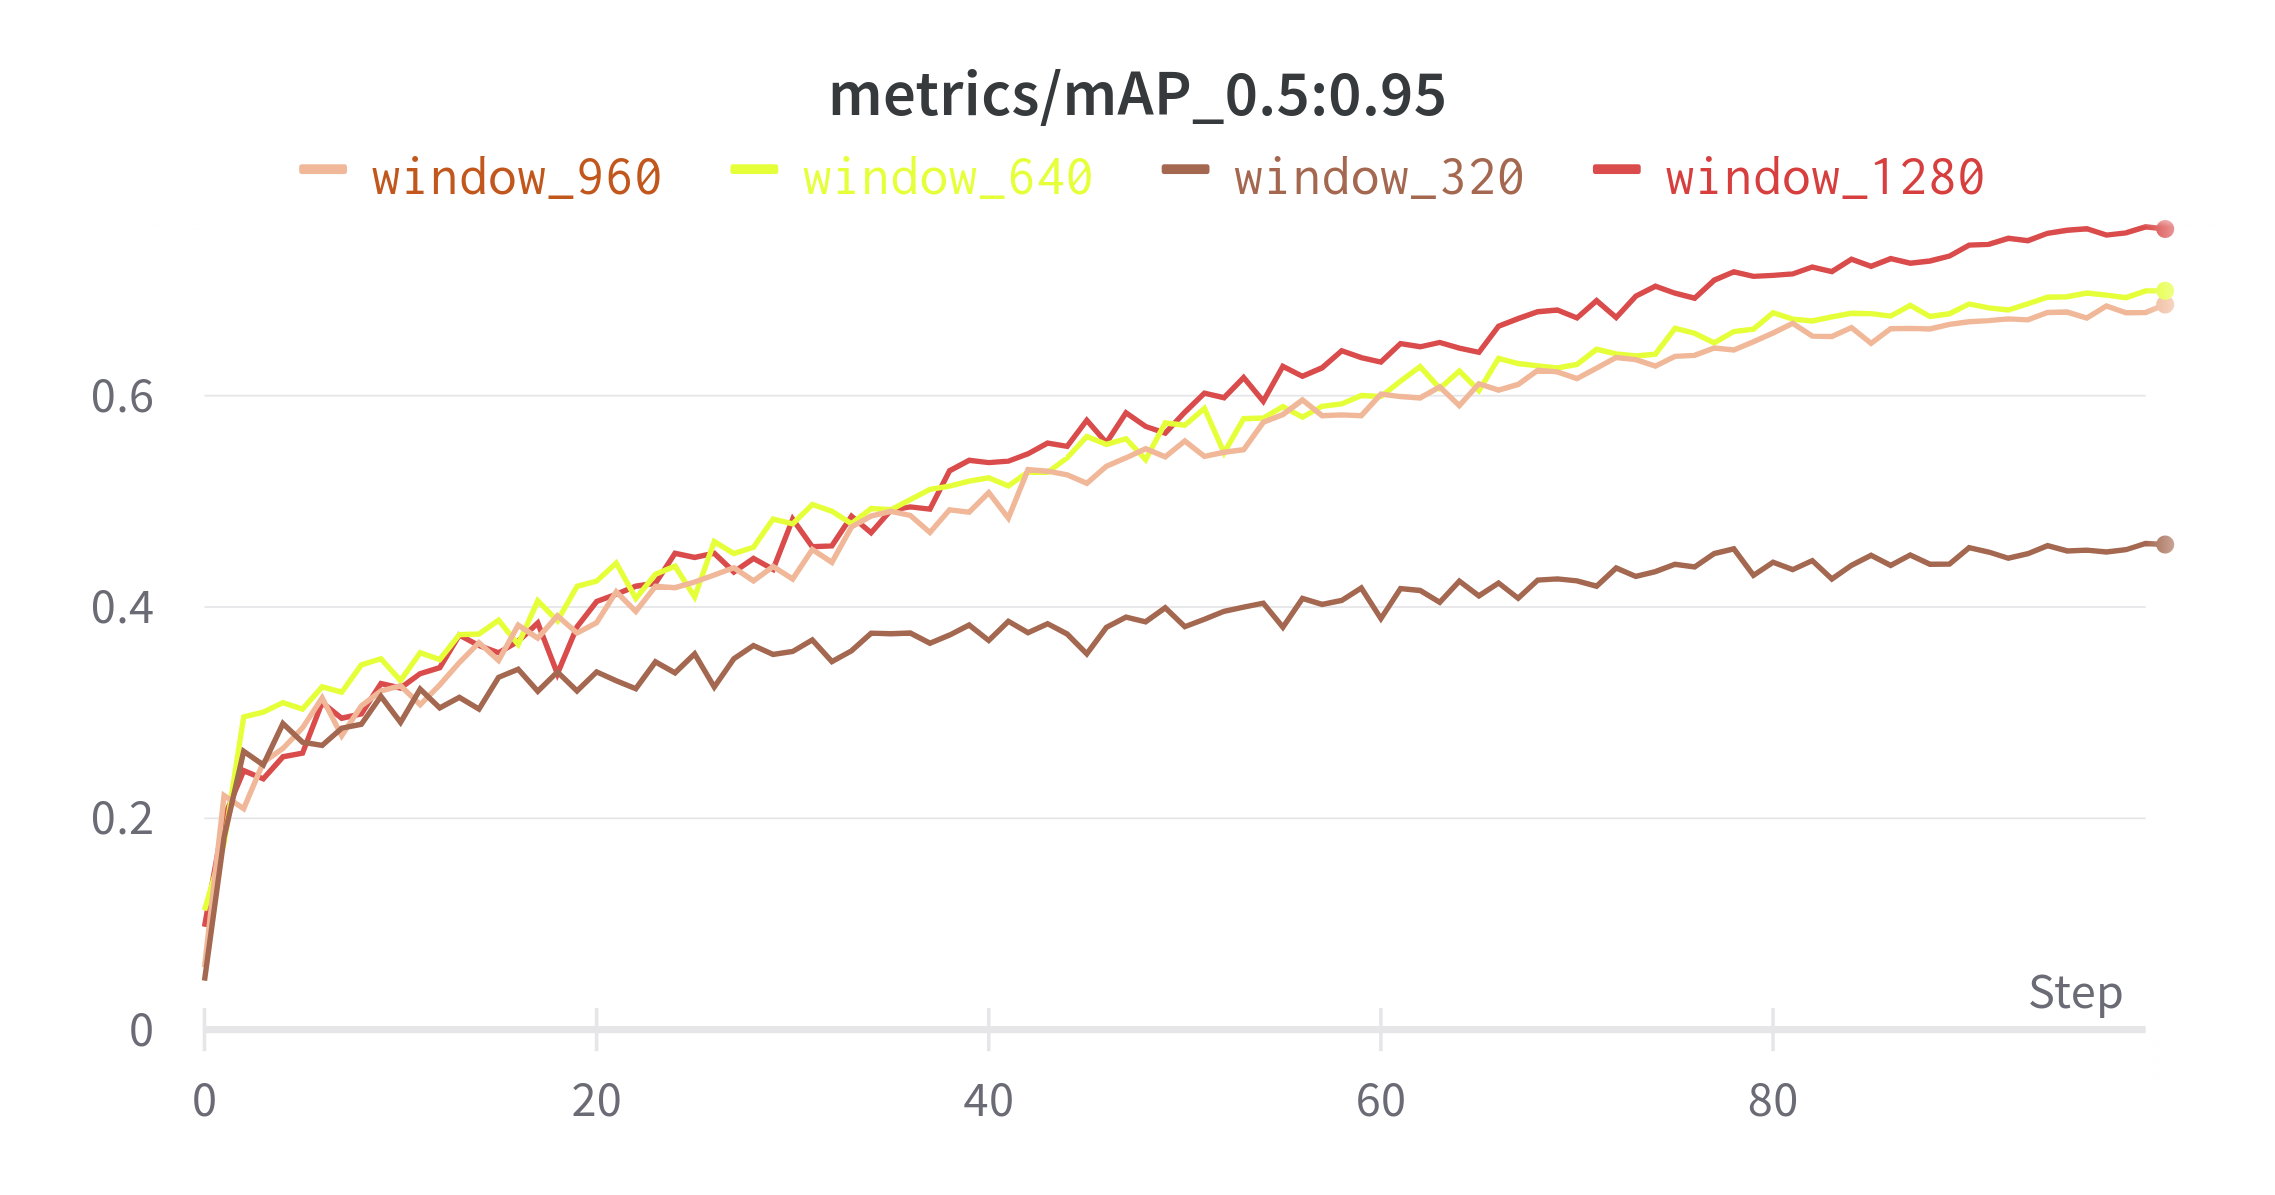
\includegraphics[width=\textwidth]{images/map_win_size}
\caption{mAP@0.5:0.95 for different window sizes}
\end{figure}

 Bigger windows might have the advantage of capturing more context information, but the drawback is the longer training time as seen in figure \ref{fig:win_train_times}. One naive way to add more context information is to simply keep more background windows with the hope of capturing informative backgrounds, but multiple experiments with different percentage of backround images did not improve the metrics. The problem was that only background images of printed surface have the potential to teach the model something relevant and keeping random background images in the dataset proved not help in any way. With this mind, a new way of keeping background information has been found: Let's say that the desired window size is 320x320. First a dataset \textit{A} with window size of 640x640 is generated and all the background windows are removed. After that, a dataset \textit{B} is obtained by spliting each window from dataset \textit{A} in 4 smaller 320x320 windows. This time all the background windows are kept. The general idea is that it is more likely to find printed regions near a scratch. Training on this new dataset B takes on average 2-3 times longer to train than on a simple 320x320 dataset with 0-10\% background images. \\

\begin{figure}
  \begin{tabular}{|c|c|}
  \hline
  window size & epoch time (in seconds) \\
  \hline
  320x320 & 16 \\
  \hline
  640x640 & 35 \\
  \hline
  960x960 & 40 \\
  \hline
  1280x1280 & 102 \\
  \hline
  \end{tabular}
  \caption{Epoch time for the same dataset, but with different window sizes.}
  \label{fig:win_train_times}
\end{figure}


 One interseting fact for this approach was that training on dataset \textit{B} produced metrics very close to ones from training on dataset \textit{A}. This concept was tested on multiple window sizes for consistency. \\


 \subsubsection{Rectangular training and other caveats}
 TODO
with --rect no shuffling, image padded, no mosaic or cut-mix



\subsection{Mosaic and Cut-Mix}


\subsection{Translate and Scale}

\subsection{Create Custom Online Augmentation}

\subsection{Stretches and Squeezes}
Luckily the presented dataset had generally a good distribution of the lengths of scratches, but an interesting research topic was the robustness of the trained model.
TODO plot distribution \\

 How well does YOLOv5 perform at detecting longer scratches, if it was trained only on shorter scratches? And vice-versa? A


TODO talk about artifical examples?? \\

\subsubsection{Constrast}



\subsection{Hyperparameter Optimizations}

\subsubsection{Model Size}

\subsubsection{Hyperparameter evolution}

\subsubsection{Batch Size}
The official documentation recommends that training should be performed on the biggest batch size possible in order to produce the best batch normalization statistics, but meanwhile on the official Github repository the developers suggest that YOLOv5 is batch agnostic (TODO source). For the sake of finding the truth, multiple experiments with varying batch sizes have been made. The results were that for batch sizes up to 64 the map@0.5:0.95 metric was in favour of bigger batch sizes. Other metrics had no tangible differences. Bigger batches required more than 2 GPUs or compromising to a smaller window size. \\
TODO show results \\

\subsubsection{Learning Rate and Gradient}
The initial experiments showed high jumps after each epoch, so a switch from the standard stochastic gradient descent to AdamW has been made. The documentation recommends for AdamW to change the learning rate from 0.01 to 0.001, but a step size of 0.0001 showed a more stable evolution from epoch to epoch.
TODO maybe show some results

\subsubsection{Loss Function}


\subsubsection{IoU threshold}


TODO obiective dataset:
scratches position
scratches length should have variety (prin stretch si prin window cuts)
scratch strength variety (sa inventez ceva)

easy source code modifications (la metrics mai ales)
dataset format
dataset postprocessing (black border)
